
%Copyright (C) 2016 by Krishneel@JSK Lab, The University of Tokyo

\documentclass{standalone}

\usepackage{graphicx}
\usepackage{float}
\floatstyle{boxed} 
\restylefloat{figure}

\begin{document}

\subsection{Setup of Testbed}
We have started to operate all tasks simultaneously, as shown in Fig.\ref{fig:grand}. The fundamental performances of each task have been comfirmed.

 \subsection{Future Work}
We plan to establish the mutual communication among the field robots to enhance the performance. For instance, we will use the image data from the robot of task2 to recognize the truck for task1 and objects of task3, and vice versa.
 
\begin{figure}[h]
    \begin{center}
      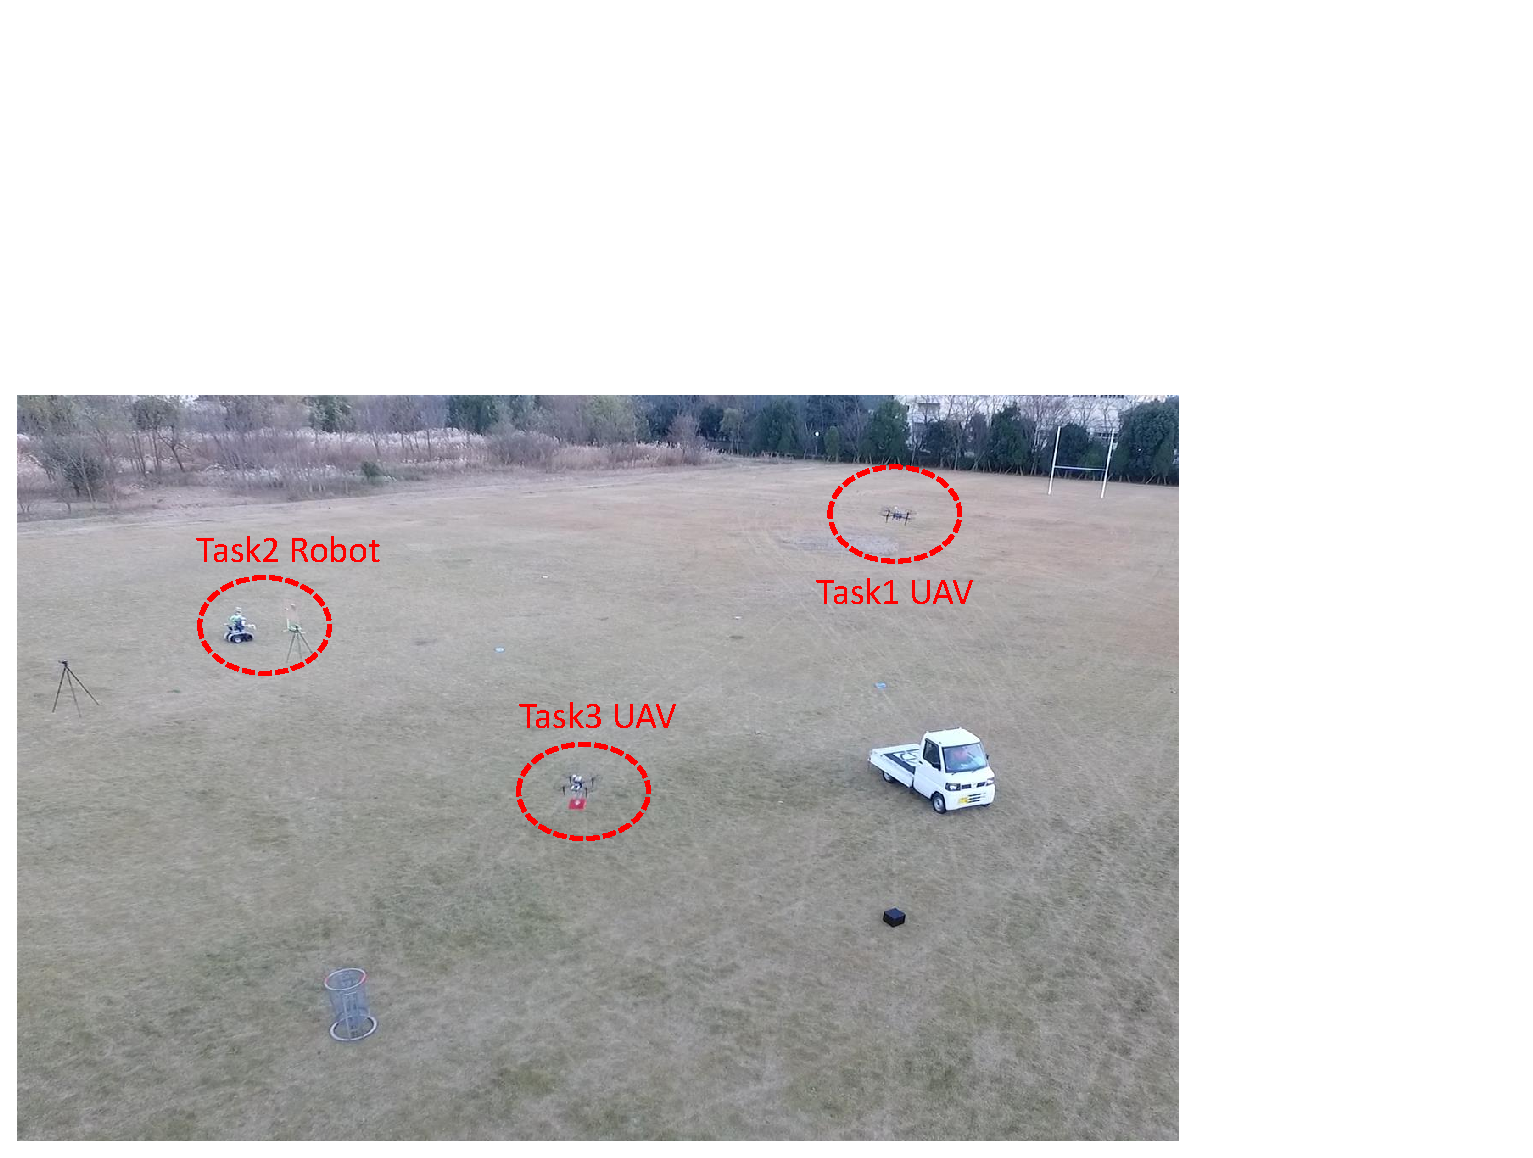
\includegraphics[clip, bb= 0 0 560 360, width=1.0\columnwidth]{sections/grand/images/grand_challenge.eps}
    \end{center}
   \caption{Experiment of Ground Challenge in Kasihiwa, Chiba, Japan}
   \label{fig:grand}
 \end{figure}


\end{document}
